\section{The Apparent Result}
\label{sec:apparent}

\subsection{The naive quantile profile}

Table~\ref{tab:qlp} and Figure~\ref{fig:irf} report the headline estimates
of Equation~\eqref{eq:qlp}. On impact, the response of the first percentile
is $\beta_0(0.01) = \BetaQoneHzero$, strongly significant under the
tail-appropriate block-bootstrap inference, while the median barely moves
($\beta_0(0.50) = \BetaMedHzero$). The tail response is
\RatioTailMedImpact{} times the median response. The left tail also appears
to respond more than the right, with $|\beta_0(0.01)|/|\beta_0(0.95)| =
\GapLrImpact$ on impact.

At first reading this is what the leverage-cycle prior\footnote{The
view we deconstruct is actively held, not a strawman built for contrast.
Alongside the leverage-cycle theory cited here it rests on the fire-sale
tradition \citep{shleifer1992}, finds empirical grounding for DeFi in the
leveraging spirals documented by \citet{perez2021} and the systemic
fragility analyzed by \citet{lehar2022}, and is monitored by the official
sector as a financial-stability concern \citep{oecd2023,fsb2023}.} predicts
\citep{geanakoplos2010,brunnermeier2009}: a liquidation shock depresses the
crash quantile of returns far more than the center, and more than the
upside. It is, term for term, the Growth-at-Risk pattern of
\citet{adrian2019}, with the lower tail responding where the mean is blind
(our OLS control regression sees nothing at any horizon). And it is produced
by an established estimator \citep{han2024}, not an exotic one. The
reservation entered below is never about the \emph{existence} of
$\beta$; it is about its \emph{interpretation}.

\begin{table}[t]
\centering
\caption{Quantile local projections: $\beta_h(\tau)$ of cumulative ETH
returns on the liquidation shock.}
\label{tab:qlp}
% GENERATED by scripts/paper/make_tables.py — DO NOT EDIT
% fragment only: wrap in \begin{table} + caption in the manuscript
\begin{tabular}{lcccccc}
\toprule
$\tau$ & $h=0$ & $h=1$ & $h=3$ & $h=6$ & $h=12$ & $h=24$ \\
\midrule
0.01 & -0.032 & -0.087 & -0.105 & -0.160 & -0.241 & -0.213 \\
0.05 & -0.019 & -0.045 & -0.046 & -0.079 & -0.102 & -0.116 \\
0.10 & -0.013 & -0.030 & -0.034 & -0.043 & -0.061 & -0.095 \\
0.50 & 0.002 & 0.006 & 0.010 & 0.014 & 0.032 & 0.038 \\
0.90 & 0.014 & 0.028 & 0.038 & 0.047 & 0.070 & 0.102 \\
0.95 & 0.018 & 0.031 & 0.044 & 0.041 & 0.077 & 0.116 \\
\bottomrule
\end{tabular}

\begin{minipage}{0.92\textwidth}
\vspace{2pt}
{\scriptsize \emph{Notes:} Locked specification (seven regressors,
Section~\ref{sec:method}); $N \approx \Nobs$. Point estimates; tail
inference is by moving-block bootstrap (Figure~\ref{fig:irf} displays the
95\% band on $\tau=0.01$), kernel standard errors being unreliable at
extreme quantiles (Appendix Table~\ref{tab:seratio}).}
\end{minipage}
\end{table}

\begin{figure}[t]
\centering
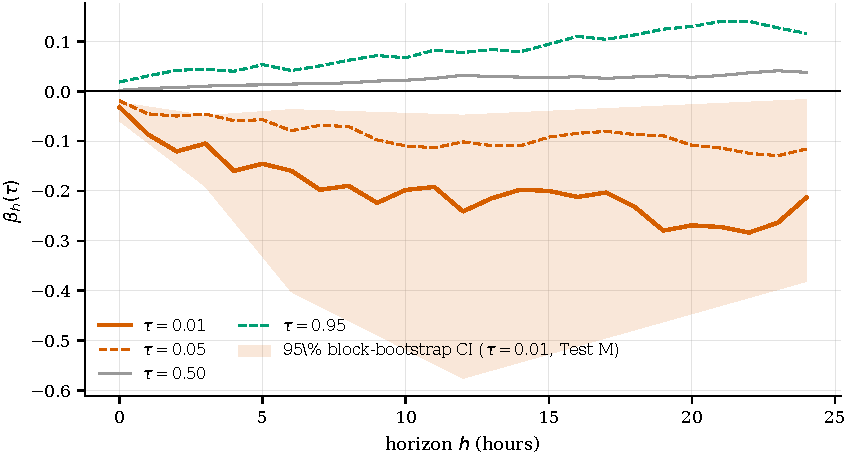
\includegraphics[width=\textwidth]{../paper/figures/fig3_qlp_irf}
\caption{Quantile local-projection responses $\beta_h(\tau)$ with the 95\% block-bootstrap band on $\tau = 0.01$ (headline specification). The fan widens and the lower tail deepens with the horizon.}
\label{fig:irf}
\end{figure}

\subsection{The deepening profile}

The tail coefficient deepens almost monotonically with the horizon:
$\BetaQoneHzero$ on impact, $\BetaQoneHone$ at one hour, $\BetaQoneHtwelve$
at twelve, with a plateau near $\BetaQoneHtwentyfour$ at twenty-four
(Table~\ref{tab:qlp}). An effect that grows as the window lengthens reads
naturally as the footprint of a spiral, the shock propagating and
self-reinforcing, which is the reading a leverage-cycle prior
invites. We flag, without yet arguing, that the left-hand side at $h > 0$
is an overlapping cumulative return, a construction whose tail behavior
under the null deserves dedicated scrutiny, and receives it in
Section~\ref{sec:deconstruction}
\citep{hodrick1992,boudoukh2008,neuberger2021,farago2023}.

\subsection{The apparent robustness}

The pattern checks every box a referee would ask for. The block-bootstrap
band on $\tau = 0.01$ excludes zero at every horizon (on impact
$[\TestMLoHzero, \TestMHiHzero]$; at twelve hours
$[\TestMLoHtwelve, \TestMHiHtwelve]$; at twenty-four
$[\TestMLoHtwentyfour, \TestMHiHtwentyfour]$; $1{,}000$ replications). The
sign and significance survive a battery of conventional robustness checks,
including placebo assets, alternative shock definitions, subperiod and
episode exclusions, and monotonicity across quantiles, reported in
Appendix~\ref{app:robustness}. And the direct effect survives Bonferroni
correction in full: 12 of 12 cells of the reported $\tau\times h$ grid and
6 of 6 of the quantile grid. By the usual standards of empirical asset pricing, this is a
robust result.

Two cautions temper the checklist. Multiple-testing corrections guard
against \emph{noise}, not against \emph{misinterpretation}. Surviving
Bonferroni says the effect is not sampling luck; it does not say the effect
is a downside skew rather than a symmetric volatility response read through
extreme quantiles. And at $\tau = 0.01$ the extremal quantile literature
counsels explicit caution on point estimates
\citep{chernozhukov2005,chernozhukov2011}; tail inference here therefore
rests on interval estimates, from the moving-block bootstrap motivated on
separate grounds in Section~\ref{sec:method-inference}.

\subsection{The leverage interaction}
\label{sec:apparent-crack}

The leverage-cycle story makes a sharper prediction than ``liquidations
depress the tail'': amplification should be \emph{stronger when leverage is
high}. The interaction term $\delta_h(\tau)$, the specification's direct
embodiment of that prediction, is null across the tail-quantile grid. At $\tau = 0.01$ the
bootstrap interval straddles zero at every horizon (on impact
$[\IntCILoHzero, \IntCIHiHzero]$; at twelve hours
$[\IntCILoHtwelve, \IntCIHiHtwelve]$), the sign is unstable across
resamples, and the Bonferroni family verdict is 0 of 6. This is not a
nuance to be excused. The one mechanism-specific term in the regression
fails on the tail grid, while the mechanism-agnostic direct term looks
spectacular. The leverage-cycle reading already has a hole in it.

We are careful about what this null does and does not establish. Unlike the
direct effect, the interaction is estimated with little precision: the
bootstrap interval is wide and its sign flips across resamples, so the
smallest leverage amplification it could detect at conventional power,
\MdeDeltaHzero{} at impact, is a multiple of the direct effect itself,
roughly \MdeDeltaRatioMin{} to \MdeDeltaRatioMax{} times it, not a fraction
of it. The 0/6 verdict
is therefore best read as the \emph{absence of any detectable}
leverage-specific amplification rather than as a tight bound on its
magnitude, a hole in the mechanism story rather than a measured zero. The
decisive, quantified bounds in this paper attach to the symmetric-scale and
down-minus-up asymmetry objects (Section~\ref{sec:survives}), where
standardizing by predetermined volatility cancels the common scale and
sharpens the test; the interaction inherits no such cancellation, which is
why it stays wide. The interaction is, however, not null at the centre of the
distribution: at the median it is significantly negative at the twelve- to
twenty-four-hour horizons ($\delta_{12}(0.50) = \DeltaIxnMedHtwelve$,
$p = \DeltaIxnMedHtwelveP$), so high-leverage hours shift the shock's median
response downward. That is a level effect on the centre of the return
distribution, not the downside-tail amplification the leverage-cycle prior
predicts, and it is orthogonal to the down-minus-up asymmetry this paper
bounds; it is consistent with a liquidation channel that is real and locally
disruptive yet does not aggregate into tail fragility
(Section~\ref{sec:mechanisms}).

\subsection{Summary of the apparent result}

Taken together: a direct effect \RatioTailMedImpact$\times$ the median on
impact, deepening to \BetaQoneHtwelve{} by twelve hours, robust across a
battery of robustness checks, surviving multiple-testing correction in full, and
a mechanism term that is cleanly null. The question that the next
section answers is the one this contrast forces. Is the real, robust
direct effect a genuine \emph{downside} response, or the same symmetric
volatility that thickens \emph{both} tails, misread by a quantile local
projection on overlapping cumulative returns?